\begin{figure*}[hbtp]
  \centering
  \subfigure[Initial graph]{
    \label{fig:about-frontier-df1}
    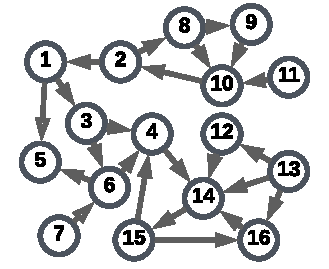
\includegraphics[width=0.23\linewidth]{out/about-frontier-11.pdf}
  }
  \subfigure[Marking initial affected vertices (DF)]{
    \label{fig:about-frontier-df2}
    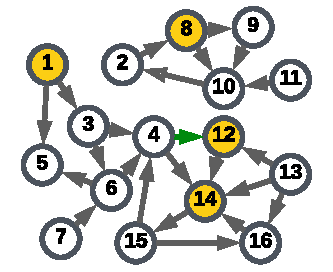
\includegraphics[width=0.23\linewidth]{out/about-frontier-32.pdf}
  }
  \subfigure[After first iteration (DF)]{
    \label{fig:about-frontier-df3}
    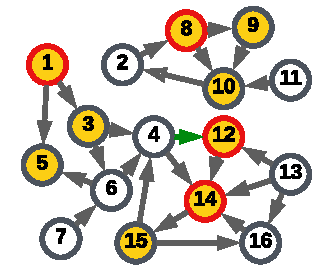
\includegraphics[width=0.23\linewidth]{out/about-frontier-33.pdf}
  }
  \subfigure[After second iteration (DF)]{
    \label{fig:about-frontier-df4}
    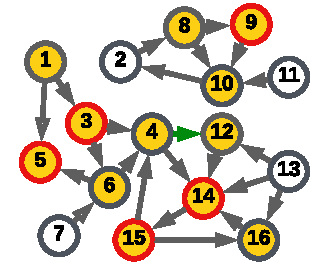
\includegraphics[width=0.23\linewidth]{out/about-frontier-34.pdf}
  } \\[2ex]
  \subfigure[Initial graph]{
    \label{fig:about-frontier-dfp1}
    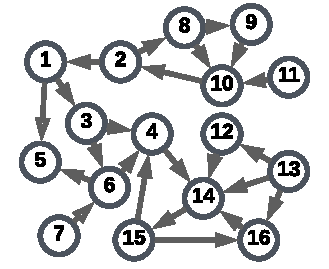
\includegraphics[width=0.23\linewidth]{out/about-frontier-11.pdf}
  }
  \subfigure[Marking initial affected vertices (DF-P)]{
    \label{fig:about-frontier-dfp2}
    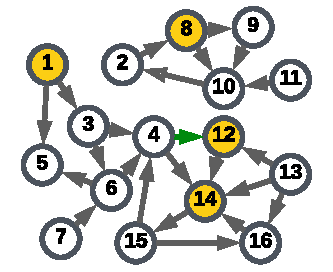
\includegraphics[width=0.23\linewidth]{out/about-frontier-32.pdf}
  }
  \subfigure[After first iteration (DF-P)]{
    \label{fig:about-frontier-dfp3}
    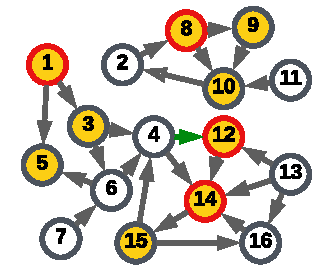
\includegraphics[width=0.23\linewidth]{out/about-frontier-33.pdf}
  }
  \subfigure[After second iteration (DF-P)]{
    \label{fig:about-frontier-dfp4}
    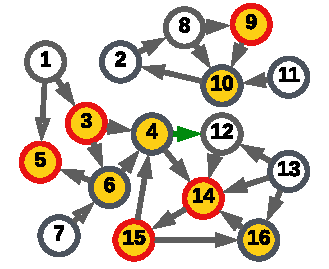
\includegraphics[width=0.23\linewidth]{out/about-frontier-44.pdf}
  } \\[2ex]
  \subfigure[Initial graph]{
    \label{fig:about-frontier-dt1}
    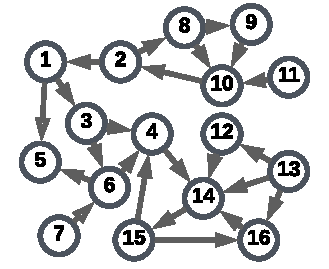
\includegraphics[width=0.23\linewidth]{out/about-frontier-11.pdf}
  }
  \subfigure[Marking affected vertices (DT)]{
    \label{fig:about-frontier-dt2}
    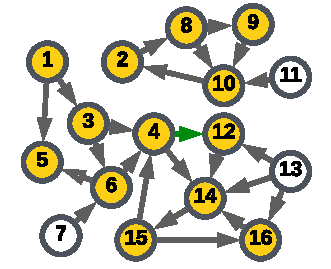
\includegraphics[width=0.23\linewidth]{out/about-frontier-22.pdf}
  }
  \subfigure[After first iteration (DT)]{
    \label{fig:about-frontier-dt3}
    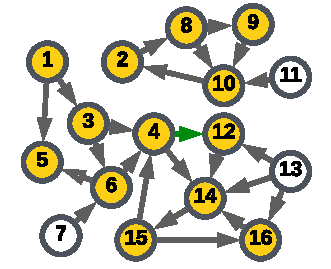
\includegraphics[width=0.23\linewidth]{out/about-frontier-22.pdf}
  }
  \subfigure[After second iteration (DT)]{
    \label{fig:about-frontier-dt4}
    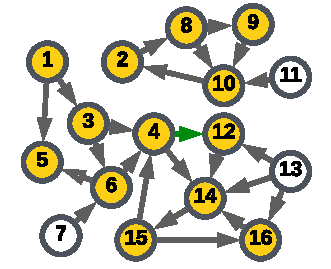
\includegraphics[width=0.23\linewidth]{out/about-frontier-22.pdf}
  } \\[-2ex]
  \caption{An example showcasing our improved \textit{Dynamic Frontier (DF)} and \textit{Dynamic Frontier with Pruning (DF-P)} approaches, in subfigures (a)-(d) and (e)-(h) respectively, in contrast to the \textit{Dynamic Traversal (DT)} approach, shown in subfigures (i)-(l).}
  \label{fig:about-frontier}
\end{figure*}

\ignore{An example showcasing our improved \textit{Dynamic Frontier (DF)} and \textit{Dynamic Frontier with Pruning (DF-P)} approaches. The initial graph has $16$ vertices and $23$ edges. The graph is updated with an edge insertion $(4, 12)$ and an edge deletion $(2, 1)$. Consequently, with DF and DF-P PageRank, the outgoing neighbors of vertices $2$ and $4$ (i.e., vertices $1$, $8$, $12$, and $14$) are marked as affected (shown with yellow fill). In the first iteration, when computing the ranks of these affected vertices, it is observed that the relative change in rank of vertices $1$, $8$, $12$, and $14$ exceeds the frontier tolerance $\tau_f$ (indicated with a red border). Therefore, their outgoing neighbors (i.e., vertices $3$, $5$, $9$, $10$, $14$, and $15$) are also marked as affected, with both DF and DF-P PageRank. In the second iteration, the relative rank change of vertices $3$, $5$, $9$, $14$, and $15$ surpasses the frontier tolerance $\tau_f$, resulting in their outgoing neighbors (i.e., vertices $4$, $6$, $10$, $15$, and $16$) being marked as affected. Additionally, with DF-P PageRank, vertices $1$, $8$, and $12$ are no longer marked as affected as their relative rank change falls below prune tolerance $\tau_p$. In the following iteration, the rankings of affected vertices are updated once more. If the rank change of each vertex falls within the iteration tolerance $\tau$, indicating convergence, the algorithm terminates. In contrast, the \textit{Dynamic Traversal (DT)} approach, marks all vertices reachable from $2$ and $4$ as affected. The ranks of this set of affected vertices are then updated in each iteration.}


\subsection{Our improved Dynamic Frontier approach}
\label{sec:frontier}

When a batch update $\Delta^{t-} \cup \Delta^{t+}$ is relatively small compared to the total number of edges $|E|$, it is anticipated that only a few vertices will experience rank changes. Our improved Dynamic Frontier approach addresses this scenario by employing an incremental process to identify affected vertices.\ignore{This helps minimize unnecessary computations, as vertices distant from the updated region of the graph are unlikely to experience rank changes until the ranks of their immediate in-neighbors change. In addition, we refrain from marking a vertex's neighbors as affected if the relative change in rank of the vertex is insignificant and is likely to have a minimal impact its neighbors ranks. We also avoid unnecessary computation of ranks of vertices that have likely settled, by no longer marking them as affected if the relative change in rank of the vertex is trivial.}


\subsubsection{Explanation of the approach}
\label{sec:frontier-explanation}

Consider a batch update consisting of edge deletions $(u, v) \in \Delta^{t-}$ and insertions $(u, v) \in \Delta^{t+}$. We first initialize the rank of each vertex to that obtained in the previous snapshot of the graph.

\paragraph{Initial marking of affected vertices:}

For each edge deletion/insertion $(u, v)$, we initially mark the outgoing neighbors of the vertex $u$ in the previous $G^{t-1}$ and current graph snapshot $G^t$ as affected.

\paragraph{Incremental expansion and contraction of the set of affected vertices upon change in rank of a given vertex:}

During PageRank computation, if the rank of any affected vertex $v$ changes in an iteration by a fraction greater than the \textit{frontier tolerance} $\tau_f$, we mark its outgoing neighbors as affected. This adjustment is made because a change in a vertex's rank is expected to influence the ranks of its outgoing neighbors. Additionally, if the relative change in rank of a vertex remains below the \textit{prune tolerance} $\tau_p$, the vertex is no longer marked as affected, as its rank may have converged. However, if the rank of such a vertex has not yet settled, it may be re-marked as affected by one of its in-neighbors. This process of marking and unmarking of vertices as affected continues in every iteration.


\subsubsection{A simple example}

Figure \ref{fig:about-frontier} illustrates an example of our improved Dynamic Frontier approach. Initially, as depicted in Figure \ref{fig:about-frontier-01}, the graph comprises $12$ vertices and $16$ edges. Subsequently, Figure \ref{fig:about-frontier-02} shows a batch update applied to the original graph, involving an edge insertion from vertex $6$ to $8$ and an edge deletion from vertex $2$ to $1$. Following the batch update, we proceed with the initial step of the Dynamic Frontier approach, marking outgoing neighbors of vertices $2$ and $6$ as affected, specifically vertices $1$, $3$, $8$, and $12$. These affected vertices are highlighted with a yellow fill. It is noteworthy that vertices $2$ and $6$ are not marked as affected. This is because changes in the out-degree of a vertex does not influence its PageRank score. Subsequently, we initiate the first iteration of the PageRank algorithm.

During the first iteration (refer to Figure \ref{fig:about-frontier-03}), the ranks of affected vertices are updated. It is observed that the relative change in rank of vertices $1$, $3$, $8$, and $12$ exceeds the frontier tolerance $\tau_f$. Such vertices are indicated with a red border in the figure. In response to this, we incrementally mark the outgoing neighbors of vertices $1$, $3$, $8$, and $12$ as affected, specifically vertices $4$, $5$, $7$, $9$, $11$, and $12$. Moreover, it is observed that the relative change in rank of vertices $1$, $3$, and $8$ remains below the prune tolerance $\tau_p$. As a result, these vertices are no longer marked as affected, as it is likely the ranks of such vertices have converged. This action effectively contracts the frontier of affected vertices. However, if the rank of such a vertex has not yet converged, it may be re-marked as affected by one of its in-neighbors.

In the second iteration, shown in Figure \ref{fig:about-frontier-04}, updates are made to the ranks of affected vertices once again. Here, it is observed that the relative change in rank of vertices $5$, $9$, $11$, and $12$ exceeds the frontier tolerance $\tau_f$. Consequently, we mark the outgoing neighbors of vertices $5$, $9$, $11$, and $12$ as affected, specifically vertices $6$, $10$, and $11$. Furthermore, vertices $4$, $5$, $7$, $9$, and $12$ are no longer marked as affected, as their relative rank change falls below the prune tolerance $\tau_p$. In the next iteration, the ranks of affected vertices are updated once more. If the change in rank of each vertex remains within the iteration tolerance $\tau$, the ranks of vertices have converged, and the algorithm terminates.




\ignore{\subsection{Synchronous vs Asynchronous implementation}}

\ignore{In a synchronous implementation, separate input and output rank vectors are used, ensuring deterministic results for parallel algorithms through vector swapping at the end of each iteration. In contrast, an asynchronous implementation utilizes a single rank vector, potentially achieving faster convergence and eliminating memory copies for unaffected vertices in dynamic approaches\ignore{, but introduces non-deterministic results in parallel algorithms}.}

\ignore{To assess synchronous and asynchronous implementations for Dynamic Frontier PageRank, both are tested on batch updates (purely edge insertions) ranging from $10^{-7}|E|$ to $0.1|E|$ for Static, Naive-dynamic, Dynamic Traversal, and Dynamic Frontier PageRank. Figure \ref{fig:approach-async} depicts the average relative runtime of asynchronous implementations compared to their synchronous counterparts. Based on the results, we use the asynchronous implementations of Naive-dynamic, Dynamic Traversal, and Dynamic Frontier PageRank --- as they are faster, especially for smaller batch sizes.\ignore{This is due to a somewhat faster convergence and the absence of copy overhead (for Dynamic Traversal and Dynamic Frontier approaches).}}




\subsection{Determination of Frontier tolerance ($\tau_f$)}
\label{sec:frontier-tolerance}

We first need to determine a suitable approach for frontier expansion, and an associate frontier tolerance $\tau_f$ value that allows us to minimize processed vertices, while limiting error to that of ranks obtained with Static PageRank using the same iteration tolerance $\tau$. For this, we experiment with three approaches. These include marking neighbors of a vertex as affected, based on change in rank of the vertex $\Delta r$, change in its contribution factor $\Delta r/d$, or relative change in its rank $\Delta r/r$. Here, $\Delta r$ is the rank change, $d$ is the out-degree, and $r$ is the vertex's \texttt{max} rank (the maximum of its previous and current rank values).

For $\Delta r$ and $\Delta r/d$, we adjust $\tau_f$ from $\tau$ to $\tau/10^5$; and for $\Delta r/r$, we adjust it from $0.1$ to $10^{-6}$. This is done on real world dynamic graphs, shown in Table \ref{tab:dataset}, with batch updates of size $10^{-5}|E_T|$. Outgoing neighbors are marked affected if the respective measure exceeds $\tau_f$. Figure \ref{fig:adjust-frontier} shows the mean speedup (with respect to Static PageRank) and rank error (compared to ranks obtained with reference Static PageRank) with each approach for frontier expansion. Results indicate that the $\Delta r/r$ approach with a $\tau_f$ of $10^{-6}$ performs best, while yielding lower error than Static PageRank.

\begin{figure*}[!hbt]
  \centering
  \subfigure[Speedup with varying Frontier tolerance $\tau_f$]{
    \label{fig:adjust-frontier--speedup}
    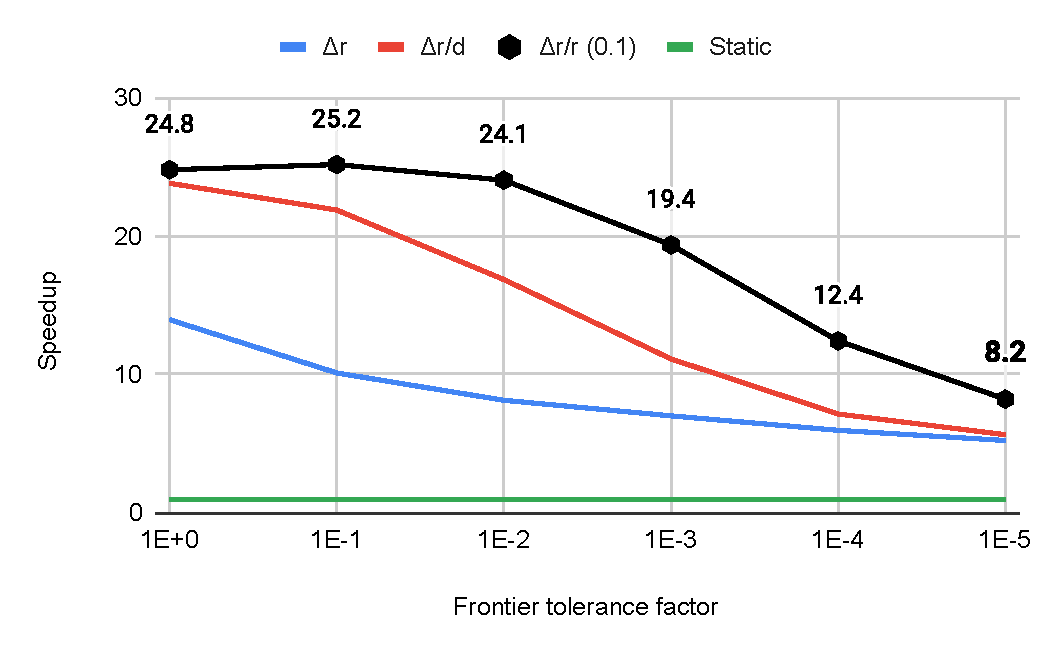
\includegraphics[width=0.48\linewidth]{out/adjust-frontier-speedup.pdf}
  }
  \subfigure[Error in ranks obtained with varying Frontier tolerance $\tau_f$]{
    \label{fig:adjust-frontier--error}
    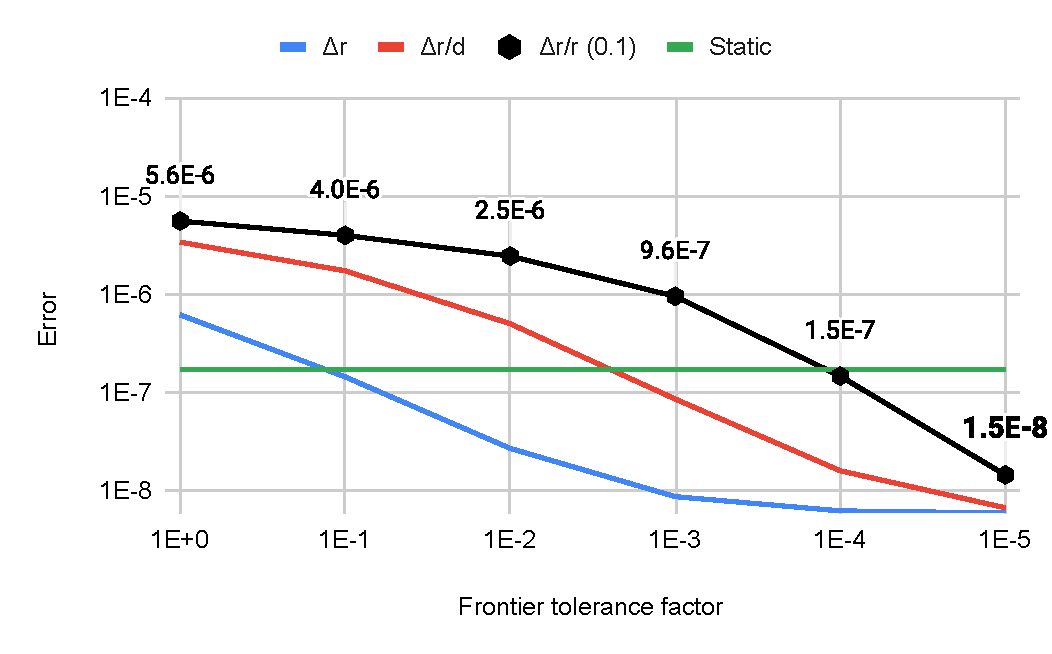
\includegraphics[width=0.48\linewidth]{out/adjust-frontier-error.pdf}
  } \\[-2ex]
  \caption{Average Speedup and Error in ranks obtained (with respect to ranks obtained with Reference Static PageRank) using \textit{Dynamic Frontier} approach, with frontier tolerance $\tau_f$ varying from $\tau$ to $\tau / 10^5$, on batch updates of size $10^{-7}|E|$ to $0.1|E|$. The figures indicate that increasing $\tau_f$ reduces runtime, but also increases the error. A Frontier tolerance $\tau_f$ of $\tau/10^4$ and $\tau/10^5$ obtain ranks with error lower than \textit{Static} PageRank, and are thus acceptable (we choose $\tau_f = \tau/10^5$ to be on the safe side).}
  \label{fig:adjust-frontier}
\end{figure*}

\begin{figure*}[!hbt]
  \centering
  \subfigure{
    \label{fig:adjust-prune--speedup}
    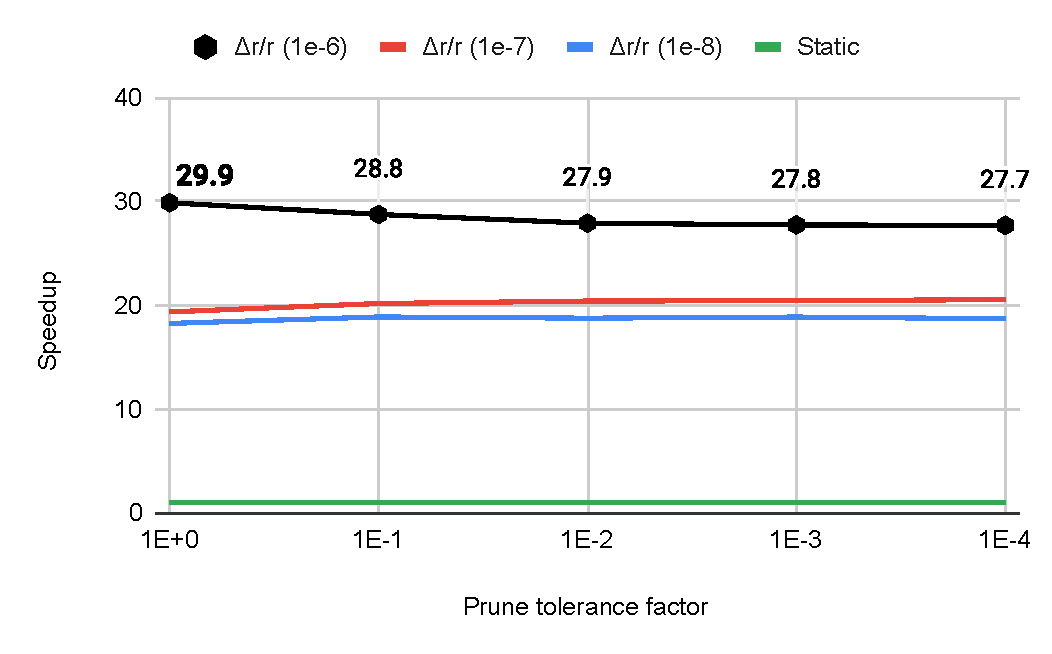
\includegraphics[width=0.48\linewidth]{out/adjust-prune-speedup.pdf}
  }
  \subfigure{
    \label{fig:adjust-prune--error}
    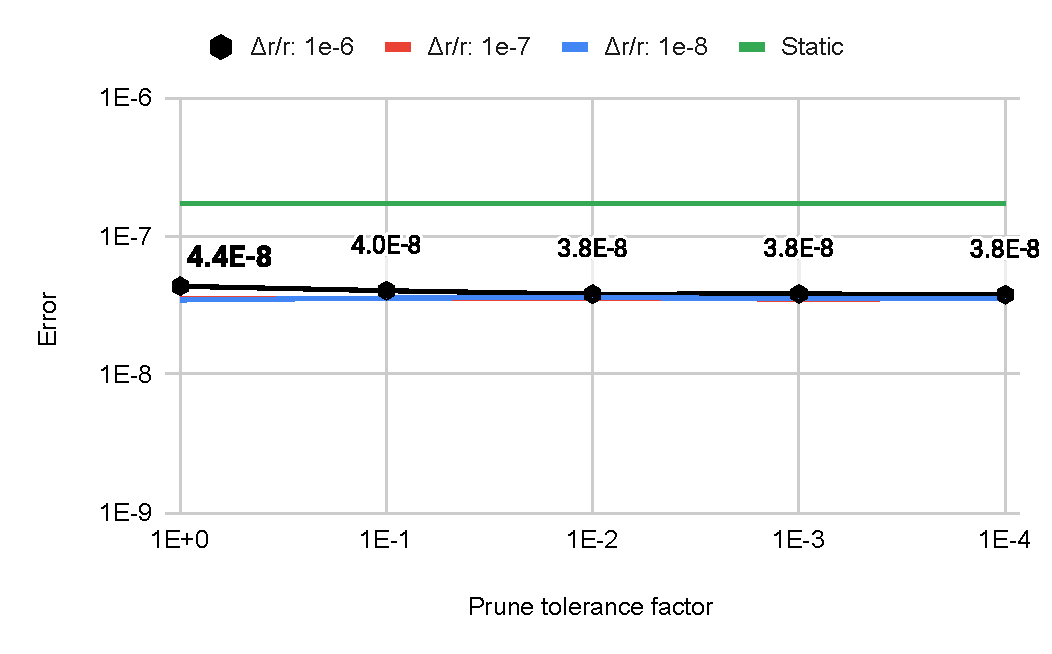
\includegraphics[width=0.48\linewidth]{out/adjust-prune-error.pdf}
  } \\[-2ex]
  \caption{Average Relative runtime with asynchronous implementations of \textit{Static}, \textit{Naive-dynamic}, \textit{Dynamic Traversal}, and \textit{Dynamic Frontier} approach compared to their respective synchronous implementations, on batch updates of size $10^{-7}|E|$ to $0.1|E|$ (right), and overall (left). The results indicate that asynchronous implementations are faster than synchronous ones, especially for smaller batch sizes. This is due to a somewhat faster convergence and the absence of copy overhead (for \textit{Dynamic Traversal} and \textit{Dynamic Frontier} approaches).}
  \label{fig:adjust-prune}
\end{figure*}

\begin{algorithm}[!hbt]
\caption{Our parallel Dynamic Frontier (DF) PageRank.}
\label{alg:frontier}
\begin{algorithmic}[1]
\Require{$G^{t-1}, G^t$: Previous, current input graph}
\Require{$\Delta^{t-}, \Delta^{t+}$: Edge deletions and insertions (input)}
\Require{$R^{t-1}, R$: Previous, current rank vector}
\Ensure{$\Delta r$: Change in rank of a vertex}
\Ensure{$\Delta R$: $L\infty$-norm between previous and current ranks}
\Ensure{$\tau, \tau_f, \tau_p$: Iteration, frontier, prune tolerance}
\Ensure{$\alpha$: Damping factor}

\Statex

\Function{dynamicFrontier}{$G^{t-1}, G^t, \Delta^{t-}, \Delta^{t+}, R^{t-1}$}
  \State $R \gets R^{t-1}$ \label{alg:frontier--initialize}
  \State $\rhd$ Mark initial affected
  \ForAll{$(u, v) \in \Delta^{t-} \cup \Delta^{t+} \textbf{in parallel}$} \label{alg:frontier--mark-begin}
    \ForAll{$v' \in (G^{t-1} \cup G^t).out(u)$}
    \State Mark $v'$ as affected
    \EndFor
  \EndFor \label{alg:frontier--mark-end}
  \ForAll{$i \in [0 .. MAX\_ITERATIONS)$} \label{alg:frontier--compute-begin}
    \State $\Delta R \gets 0$
    \ForAll{affected $v \in V^t$ \textbf{in parallel}}
      \State $r \gets (1 - \alpha)/|V^t|$
      \ForAll{$u \in G^t.in(v)$}
        \State $r \gets r + \alpha * R[u] / |G^t.out(u)|$
      \EndFor
      \State $\Delta r \gets |r - R[v]|$ \textbf{;} $\Delta R \gets \max(\Delta R, \Delta r)$
      \State $\rhd$ Prune $v$ if its relative rank change is small
      \If{$\Delta r / \max(r, R[v]) \leq \tau_p$}
        \State Mark $v$ as not affected
      \EndIf
      \State $\rhd$ Expand frontier if relative rank change is large
      \If{$\Delta r / \max(r, R[v]) > \tau_f$} \label{alg:frontier--remark-begin}
        \ForAll{$v' \in G^t.out(v)$}
          \State Mark $v'$ as affected
        \EndFor
      \EndIf \label{alg:frontier--remark-end}
      \State $\rhd$ Update rank of $v$
      \State $R[v] \gets r$
    \EndFor
    \State $\rhd$ Ranks converged?
    \If{$\Delta R \le \tau$} \textbf{break}
    \EndIf
  \EndFor \label{alg:frontier--compute-end}
  \State \ReturnInline{$R$} \label{alg:frontier--return}
\EndFunction
\end{algorithmic}
\end{algorithm}




%% Requires (parameters):
% G(V, E): a directed unweighted graph
% R: initial ranks (1/N for static)

%% Parameter values:
% MAX\_ITERATIONS = 500
% DAMPING\_FACTOR = 0.85
% TOLERANCE = 10^-10





\subsection{Determination of Prune tolerance ($\tau_p$)}
\label{sec:prune-tolerance}

We now measure a suitable value for prune tolerance $\tau_p$ for the best approach of frontier expansion $\Delta r/r$ with a frontier tolerance $\tau_f$ of $10^{-6}$, as identified in Section \ref{sec:frontier-tolerance}. For this, we adjust $\tau_p$ from $\tau_f$ to $\tau_f/10^5$. In addition, we also experiment with $\tau_f$ of $10^{-7}$ and $10^{-8}$ to be on the safe side. This is done on real world graphs, with batch updates of size $10^{-5}|E_T|$ (as earlier). A vertex is marked as unaffected, if its relative rank change $\Delta r/r$ lies within $\tau_p$.

Figure \ref{fig:adjust-prune} illustrates the mean speedup (compared to Static PageRank) and error in ranks obtained (with respect to ranks from reference Static PageRank, see Section \ref{sec:measurement}) with each $\tau_f$ for frontier expansion. The figure indicates that the $\Delta r/r$ approach with a $\tau_f$ of $10^{-6}$ and a $\tau_p$ of $\tau_f = 10^{-6}$ performs the best, while obtaining ranks with lower error than Static PageRank.




\subsection{Our DF-PageRank implementation}

Algorithm \ref{alg:frontier} shows the implementation of our improved Dynamic Frontier (DF) PageRank approach. It takes as input the previous $G^{t-1}$ and current $G^t$ snapshot of the graph, edge deletions $\Delta^{t-}$ and insertions $\Delta^{t+}$ in the batch update, the previous rank vector $R^{t-1}$, and returns as output, the updated ranks $R$.

The algorithm begins by initializing the current rank vector $R$ with the previous rank vector $R^{t-1}$ (line \ref{alg:frontier--initialize}), and marking the initially affected vertices based on edge deletions $\Delta^{t-}$ and insertions $\Delta^{t+}$ in parallel (lines \ref{alg:frontier--mark-begin}-\ref{alg:frontier--mark-end}). It then iteratively computes the rank $R[v]$ for each affected vertex $v$ (lines \ref{alg:frontier--compute-begin}-\ref{alg:frontier--compute-end}). This computation is performed in parallel, considering the incoming edges $G^t.in(v)$. The algorithm checks if the relative change in rank $\Delta r / \max(r, R[v])$ exceeds the frontier tolerance $\tau_f$, marking out-neighbor vertices as affected if so. Additionally, if the relative change in rank lies within the prune tolerance $\tau_p$, the vertex $v$ is marked as not affected. The iteration continues until either the maximum change in ranks $\Delta R$ falls below the iteration tolerance $\tau$, or the maximum number of iterations $MAX\_ITERATIONS$ is reached. Finally, the algorithm returns the final rank vector $R$ (line \ref{alg:frontier--return}).

In a push-based approach for PageRank computation, each thread calculates and sums the outgoing PageRank contribution of its vertex to its neighbors, necessitating atomic updates. In contrast, with a pull-based approach, each vertex's rank is updated through a single write by a thread \cite{verstraaten2015quantifying}. We find this to be more efficient and employ it for all implementations. Furthermore, we employ an asynchronous implementation of DF-PageRank, using a single rank vector, for potentially faster convergence and elimination of memory copies for unaffected vertices. This, based on our previous research \cite{sahu2024incrementally}, outperforms synchronous implementations, especially with smaller batch sizes. Additionally, we utilize asynchronous implementations of Naive-dynamic (ND) and Dynamic Traversal (DT) PageRank.




% Dynamic Frontier (DF) approach
% Adjusting tolerance, Frontier tolerance, Mark DelRank / DelContrib
% Dynamic Frontier optimizations
% Edge-balanced approach (Chunk size)
